% Source: public/notes/物工/問題/2020ap_exam.pdf, PDF pp. 22--23.
\documentclass[11pt,a4paper]{article}
\usepackage[margin=24mm]{geometry}
\usepackage{fontspec}
\usepackage{xeCJK}
\setCJKmainfont{HaranoAjiMincho-Regular.otf}
\setCJKsansfont{HaranoAjiGothic-Medium.otf}
\usepackage{amsmath,amssymb}
\usepackage{tikz}
\setlength{\parindent}{1em}
\setlength{\parskip}{0.35em}
\title{物理工学専攻 院試解答集\\2020年 物理学 第4問}
\author{政岡凜太郎}
\date{}
\begin{document}
\maketitle

\section*{[1] 静的な双極子ポテンシャル}
点1,2の位置は $z=\pm l/2$ なので、$r_\pm=(r^2\mp rl\cos\theta+l^2/4)^{1/2}$ である。$l/r$ の一次まで
\[
\frac1{r_+}-\frac1{r_-}=\frac{l\cos\theta}{r^2}+O(l^3/r^4).
\]
従って $q l=\alpha_0E_0$ を用いれば
\[
\varphi=\frac{\alpha_0E_0\cos\theta}{4\pi\varepsilon_0r^2},\qquad
\boxed{C=0,\quad D=1}.
\]

\section*{[2] 遅延ポテンシャル}
$\tau=t-r/c$ とおくと、$r_\pm\simeq r\mp(l/2)\cos\theta$ より
\[
q(t-r_\pm/c)l=\alpha_0E_0\cos\!\left(\omega_0\tau\pm\frac{\omega_0l\cos\theta}{2c}\right)
\simeq \alpha_0E_0\left[\cos(\omega_0\tau)\mp\frac{\omega_0l\cos\theta}{2c}\sin(\omega_0\tau)\right].
\]
また $1/r_\pm\simeq r^{-1}\pm l\cos\theta/(2r^2)$. 代入すると
\[
\varphi=\frac{\alpha_0E_0\cos\theta}{4\pi\varepsilon_0}
\left[ -\frac{\omega_0}{cr}\sin(\omega_0\tau)+\frac1{r^2}\cos(\omega_0\tau)\right],
\]
ゆえに
\[
\boxed{F=-\frac{\omega_0}{c}\sin(\omega_0\tau),\qquad G=\cos(\omega_0\tau)}.
\]

\section*{[3] ベクトルポテンシャル}
$\boldsymbol e_z=\cos\theta\boldsymbol e_r-\sin\theta\boldsymbol e_\theta$ かつ $\dot p(\tau)=-\alpha_0E_0\omega_0\sin(\omega_0\tau)$ より
\[
\boxed{\boldsymbol A=-\frac{\alpha_0E_0\omega_0}{4\pi\varepsilon_0c^2r}\sin(\omega_0\tau)
(\cos\theta\boldsymbol e_r-\sin\theta\boldsymbol e_\theta)}.
\]

\section*{[4] スカラーポテンシャルの勾配}
放射場の次数だけを保つ。遅延時刻$\tau=t-r/c$を用いると、例えば
\begin{equation}
 \partial_r\frac{\sin(\omega_0\tau)}r
 =-\frac{\omega_0\cos(\omega_0\tau)}{cr}
 -\frac{\sin(\omega_0\tau)}{r^2}
\end{equation}
であり、遅延引数の微分から$1/r$項が生じる。角度微分は$1/r^2$にとどまる。
\[
\boxed{\nabla\varphi=\frac{\alpha_0E_0\omega_0^2}{4\pi\varepsilon_0c^2r}
\cos\theta\cos(\omega_0\tau)\boldsymbol e_r+O(r^{-2})}.
\]

\section*{[5] 放射電場と磁束密度}
時間微分は $\partial_t\boldsymbol A=-\alpha_0E_0\omega_0^2\cos(\omega_0\tau)(\cos\theta\boldsymbol e_r-\sin\theta\boldsymbol e_\theta)/(4\pi\varepsilon_0c^2r)$. その動径成分は $-\nabla\varphi$ の動径成分と相殺し、
\[
\boxed{\boldsymbol E=-\frac{\alpha_0E_0\omega_0^2}{4\pi\varepsilon_0c^2r}
\sin\theta\cos(\omega_0\tau)\boldsymbol e_\theta},\qquad
\boxed{\boldsymbol B=-\frac{\alpha_0E_0\omega_0^2}{4\pi\varepsilon_0c^3r}
\sin\theta\cos(\omega_0\tau)\boldsymbol e_\phi}.
\]
磁場の方位角成分は $B_\phi=r^{-1}\{\partial_r(rA_\theta)-\partial_\theta A_r\}$ である。$\partial_r\tau=-1/c$ により第1項から上の $1/r$ 項が生じ、第2項は $O(r^{-2})$ である。従って $B_\phi=E_\theta/c$。両場は動径方向に直交し、$\boldsymbol E\cdot\boldsymbol B=0$。

\section*{[6] ポインティングベクトルと角度分布}
$\boldsymbol e_\theta\times\boldsymbol e_\phi=\boldsymbol e_r$ なので、瞬時値は
\[
\boxed{\boldsymbol S=\frac{(\alpha_0E_0\omega_0^2)^2}{16\pi^2\varepsilon_0c^3r^2}
\sin^2\theta\cos^2(\omega_0\tau)\boldsymbol e_r}.
\]
従って距離依存は $r^{-2}$、方位角 $\phi$ に依らない。時間平均した角度分布は $\langle|\boldsymbol S|\rangle\propto\sin^2\theta$ で、$\theta=0,\pi$ で零、$\theta=\pi/2$ で最大となる。下図は距離 $r$ を固定した時間平均の角度分布である。左は $\theta$ 依存性、右は $\theta=\pi/2$ に固定した $\phi$ 依存性を示す。瞬時値にも同じ角度因子があり、時刻による変化は $\cos^2(\omega_0\tau)$ による。
\begin{center}
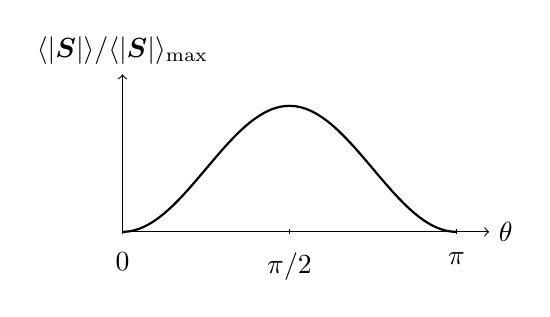
\begin{tikzpicture}[x=1.35cm,y=1.6cm]
\draw[->] (0,0)--(3.45,0) node[right] {$\theta$};
\draw[->] (0,0)--(0,1.25) node[above] {$\langle|\boldsymbol S|\rangle/\langle|\boldsymbol S|\rangle_{\max}$};
\draw[thick] plot[domain=0:pi,samples=121] (\x,{sin(deg(\x))^2});
\foreach \x/\lab in {0/0,{pi/2}/{\pi/2},pi/{\pi}} {
 \draw (\x,0.02)--(\x,-0.02) node[below=3pt] {$\lab$};
}
\end{tikzpicture}
\hspace{0.8cm}
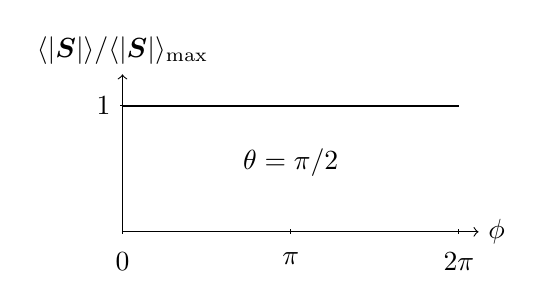
\begin{tikzpicture}[x=0.68cm,y=1.6cm]
\draw[->] (0,0)--(6.65,0) node[right] {$\phi$};
\draw[->] (0,0)--(0,1.25) node[above] {$\langle|\boldsymbol S|\rangle/\langle|\boldsymbol S|\rangle_{\max}$};
\draw[thick] (0,1)--({2*pi},1);
\foreach \x/\lab in {0/0,pi/{\pi},{2*pi}/{2\pi}} {
 \draw (\x,0.02)--(\x,-0.02) node[below=3pt] {$\lab$};
}
\draw (0.04,1)--(-0.04,1) node[left] {$1$};
\node at (pi,0.55) {$\theta=\pi/2$};
\end{tikzpicture}
\end{center}

\section*{[7] 変調された分極率と側帯波}
[2]の同じ一次展開を任意の時間依存$p(t)$に適用し、[3]の電流からのポテンシャルと合わせると
\begin{equation}
 \varphi=\frac{\cos\theta}{4\pi\varepsilon_0}
 \left[\frac{p(\tau)}{r^2}+\frac{\dot p(\tau)}{cr}\right],\qquad
 \boldsymbol A=\frac{\dot p(\tau)}{4\pi\varepsilon_0c^2r}\boldsymbol e_z.
\end{equation}
$\partial_r\tau=-1/c$より、放射場の$1/r$項は
\begin{align}
 -\nabla\varphi\big|_{1/r}
 &=\frac{\ddot p(\tau)\cos\theta}{4\pi\varepsilon_0c^2r}\boldsymbol e_r,\\
 -\partial_t\boldsymbol A
 &=-\frac{\ddot p(\tau)}{4\pi\varepsilon_0c^2r}
 (\cos\theta\boldsymbol e_r-\sin\theta\boldsymbol e_\theta).
\end{align}
動径成分が相殺するので、$\boldsymbol E=\sin\theta\,\ddot p(\tau)\boldsymbol e_\theta/(4\pi\varepsilon_0c^2r)$となる。積和公式を使うと
\begin{align*}
 p(\tau)&=E_0\left[\alpha_0\cos(\omega_0\tau)+\frac{\alpha_1}{2}\cos((\omega_0+\omega_v)\tau)+\frac{\alpha_1}{2}\cos((\omega_0-\omega_v)\tau)\right],\\
 \ddot p(\tau)&=-E_0\left[\alpha_0\omega_0^2\cos(\omega_0\tau)
 +\frac{\alpha_1}{2}(\omega_0+\omega_v)^2\cos((\omega_0+\omega_v)\tau)
 +\frac{\alpha_1}{2}(\omega_0-\omega_v)^2\cos((\omega_0-\omega_v)\tau)\right].
\end{align*}
従って
\[
\begin{aligned}
\boldsymbol E(\boldsymbol r,t)=-\frac{E_0\sin\theta}{4\pi\varepsilon_0c^2r}\Bigl[&\alpha_0\omega_0^2\cos(\omega_0\tau)\\
&+\frac{\alpha_1}{2}(\omega_0+\omega_v)^2\cos((\omega_0+\omega_v)\tau)\\
&+\frac{\alpha_1}{2}(\omega_0-\omega_v)^2\cos((\omega_0-\omega_v)\tau)\Bigr]\boldsymbol e_\theta.
\end{aligned}
\]
散乱波に含まれる正の角振動数は $\boxed{\omega_0,\ \omega_0+\omega_v,\ \omega_0-\omega_v}$ である（$\omega_v\ll\omega_0$）。
\end{document}
